
\documentclass[12pt, a4paper, english, brazil]{article}

% Sistema autor-data com títulos nas referências em negrito
% \usepackage[alf,abnt-emphasize=bf]{abntex2cite}

% \usepackage[alf,abnt-emphasize=bf,abnt-repeated-author-omit=yes,abnt-year-extra-label=yes]{abntex2cite}	% Citações padrão ABNT

% ----------------- link in the PDF
% http://tug.ctan.org/macros/latex/contrib/abntex2/doc/abntex2cite.pdf
%Usando o pacote abntex2cite autonomamente ... é preciso passar a opção carregando o pacote url antes do abntex2cite
\usepackage[hyphens]{url}
\usepackage[bookmarks=false]{hyperref}
\usepackage{hyperref}
% ----------------- link in the PDF

\usepackage[alf,abnt-emphasize=bf,abnt-repeated-author-omit=yes]{abntex2cite}

\usepackage[utf8]{inputenc}	
\usepackage[brazil]{babel}
\usepackage{graphicx,url}
\usepackage{subfigure}
\usepackage{enumitem}
\usepackage{amsfonts}
\usepackage{amsmath}

\usepackage{physics}
\usepackage{comment}

\usepackage{lscape}

\usepackage{fancyhdr}

% -
\usepackage{indentfirst}
% \graphicspath{{img/}}
%\pagestyle{empty}

\usepackage{xcolor}

\newcommand{\textRed}[1]{{{\color{red} #1}}}
\newcommand{\textBlue}[1]{{{\color{blue} #1}}}
\newcommand{\dotsBlue}{\colorbox{orange}{\textcolor{blue}{\dots}}}
\newcommand{\boxRed}[1]{\colorbox{red}{#1}}
\newcommand{\boxYellow}[1]{\colorbox{yellow}{#1}}
\newcommand{\linePage}{--------------------------------------------------------------------------------------------------------------}

\usepackage{tabularx}
\newcolumntype{L}{>{\raggedright\arraybackslash}X}
\usepackage{amssymb}% \varnothing

% -

\textwidth 16cm \textheight 23.2cm
\voffset -1.5cm \hoffset -1.4cm

\sloppy

\begin{document}

\rhead{\thepage}
\pagenumbering{arabic}

\begin{center}
	\bf{\LARGE{PROJETO DE DISSERTAÇÃO}\\ $\ $\\}
	\Large{Programa de Mestrado em Ciência da Computação\\
		Universidade Federal de Uberlândia}\\ $\ $\\
\end{center}

\begin{center}
	\bf{Aluno: João Batista Ribeiro\\ $\ $\\
		Orientador: Prof. Dr. André Ricardo Backes\\ $\ $\\
		Coorientador: Prof. Dr. Maurício Cunha Escarpinati\\ $\ $\\
		Data da formalização da coorientação no colegiado: \colorbox{yellow}{xx/xx/2021}\\ $\ $\\
		Título do Trabalho: \colorbox{yellow}{Detecção de linhas de plantio em plantações de cana-de-açúcar}\\ $\ $\\
		Data de Início como Aluno Regular: março de 2021\\ $\ $\\
		Previsão da Defesa: fevereiro de 2023\\ $\ $\\}
\end{center}

\textRed{Versão 0.2 - 06/10/2021}

\section{Introdução}

O rápido crescimento populacional, principalmente no último século, tem impulsionado a demanda por alimentos e a utilização inteligente/sustentável dos recursos naturais. Nesse contexto, a agricultura aliada tecnologia, chamada de Agricultura de Precisão (AP), busca suprir essa demanda utilizando os recursos sob medida com base nas informações coletadas. A AP engloba uma série de técnicas diferentes, como a análise espacial da área plantada, informações do solo e das plantas, permitindo aos produtores planejar e monitorar suas plantações \cite{Blasch_2020}.

A Agricultura de Precisão se tornou possível graças ao desenvolvimento e avanços de diferentes tecnologias, como o Sistema de Posicionamento Global (GPS), o uso de imagens de satélites, o desenvolvimento de novas técnicas de Processamento Digital de Imagens (PDI) e Visão Computacional, sensoriamento remoto entre outras. Isso possibilitou o desenvolvimento de metodologias, técnicas e programas que são aplicados nas várias etapas da agricultura, desde análise e preparação do solo (para determinar a escassez de determinado nutriente numa região) até a utilização de veículos autônomos para fazer a pulverização de defensivos (com quantidade específica para cada parte do talhão) e na colheita seguindo as linhas de plantio. Muitos dos avanços na AP são fortemente dependentes das tecnologias de processamento digital de imagens \cite{Bolfe_2020}.

As imagens utilizadas na AP têm variadas fontes (e.g., câmeras acopladas em Veículos Aéreos Não Tripulados (VANTs) e satélites) dependendo da aplicação e do \textit{Ground Sample Distance} (GSD) requisitado. O GSD refere-se à distância da amostra ao solo, ou seja, quanto cada pixel da imagem obtida representa da região fotografada. Assim quanto menor for o GSD, mais detalhes a imagem terá da região analisada. Satélites (com GSD em média de metros) conseguem imagem de grande regiões mais facilmente que os VANTs (GSD em média de centímetros), que necessitam de planos de voo para abranger toda região e mosaicagem para combinar as imagens obtidas \cite{Messina_2020}.

O custo das imagens de satélites depende muito da qualidade das imagens, elas possuem baixa temporalidade (imagens de uma mesma área em momentos diferentes), um baixo nível de detalhes (maior GSD) em relação aos VANTs e sofrem bastante com as condições climáticas (e.g., nuvens). Por outro lado, os VANTs geralmente têm custo baixo para aquisição das imagens, possibilitam a captura (e recaptura) das imagens sempre que necessário (alta temporalidade e disponibilidade), com grande nível de detalhes (pequeno GSD) e não sofrem muito com as nuvens devido a sua altitude de voo \cite{Candiago_2015, Delavarpour_2021}.

Uma das aplicações importantes da AP é a detecção das linhas de plantio, principalmente porque esta é utilizada como uma etapa importante para outras aplicações da AP (e.g., detecção de ervas daninhas, mapeamento e previsão de produção de safra, detecção de falhas) \cite{Hassanein_2019}. Além de ser utilizada pelos veículos autônomos para se guiarem na plantação, assim evitando o pisoteamento da cultura \cite{Doha_2021}.

A detecção de linhas de plantio é uma tarefa complexa e com vários desafios. Por exemplo, pode haver a presença de ervas daninhas com assinatura espectral e cor semelhantes a linhas da cultura, dificultando a sua detecção. Crescimento irregular da cultura, falhas no plantio, imperfeições e oclusões linha de plantio, manchas de solo e tipos diferentes na mesma plantação, presença de artefatos bloqueando a visão da linha de cultivo (e.g., árvores), sombras, além de variações nas condições climáticas e de iluminação, são exemplos de variações presentes nas imagens e que podem atrapalhar, ou mesmo comprometer, o processo de detecção  \cite{Rabab_2021, Doha_2021}.

Um dos cenários de grande utilização da Agricultura de Precisão no Brasil é no cultivo de cana-de-açúcar (\textit{Saccharum officinarum}), motivando pesquisadores (e.g., \citeonline{Souza_2017, Souza_2018, Silva_Escarpinati_Backes_2021}) e empresas (e.g., \citeonline{AERO_2017, Sensix_2020, Inforow_2021}) a desenvolverem soluções na área.

O Brasil é o maior produtor e exportador de cana-de-açúcar, com aproximadamente 10 milhões de hectares de área plantada, sendo que mundialmente esse valor é de pouco mais de 26 milhões de hectares \cite{Ritchie_2020, IBGE_2021, FAOSTAT_2021}. O seu cultivo é de grande importância para a economia brasileira devido as suas diversas aplicações. A cana-de-açúcar pode, por exemplo, ser consumida fresca na alimentação humana e forragem na alimentação animal, produção de açúcar, bebidas, energia e combustíveis. Além disso, seus subprodutos, como o bagaço e a palha, podem ser utilizados na fertilização do solo \cite{Oliveira_2018}.

A cana-de-açúcar é uma cultura semi-perene (seu manejo pode durar anos sem ser necessário um novo plantio), o que adiciona uma motivação a mais para detectar as suas linhas de plantio em relação a outras culturas (e.g., milho). Após a primeira colheira, a rebrota das soqueiras é colhida anualmente por cerca de 5 a 7 anos, ou mais \cite{Rudorff_2010}. Contudo, isso também adiciona um desafio, pois dependendo do estágio da plantação, folhas secas estão presentes no solo entre as linhas da cultura, dificultando a análise computacional \cite{Silva_2020}.

Apesar de na literatura já existirem muitos trabalhos para detectar linhas de plantio, a maioria deles são para outras culturas (e.g., milho e beterraba) ou focados em linhas retas \cite{Pereira_Junior_2020}. Além de muitos utilizarem imagens de baixíssima altitude ($\le$ 2 m), tiradas a partir do solo (manualmente ou acopladas no maquinário agrícola) ou de alta altitude (imagens de satélites) \cite{Hasan_2021}.

Outro ponto importante, atualmente não é possível encontrar (\textRed{não é uma afirmação muito forte o ``não é possível"?}) nenhum \textit{software} gratuito e de código aberto que faça a detecção das linhas de plantio corretamente (em cana-de-açúcar ou outro tipo de cultura), apenas \textit{softwares} comerciais. Assim este projeto também busca desenvolver uma metodologia de detecção das linhas de plantio que possa ser utilizada no desenvolvimento de um \textit{software}, promovendo uma democratização do conhecimento.

Considerando o cenário de grande utilização dos VANTs para obtenção de imagens para a Agricultura de precisão, a grande importância da detecção das linhas de plantio, este projeto tem como foco a detecção de linhas de plantio de cana-de-açúcar.

%\subsection{Motivação}
    % Deixar dentro da introdução
 
\subsection{Objetivos e desafios da pesquisa}
\textRed{Melhor mudar o título para objetivos? Comentei um pouco dos desafios na introdução.}
    % => Descreva claramente os desafios que o tema propõe e quais os objetivos que se pretende alcançar. Se o tema for muito abrangente, descreva os objetivos em termos de ``objetivo geral'' e ``objetivos específicos''. Cuidado com objetivos como ``desenvolver um sistema...''; ``explorar um método...'' Esses objetivos são triviais, ou seja, uma vez desenvolvido o sistema ou explorado o método, independente dos resultados, o objetivo foi atingido. Prefira verbos como: ``contribuir'', ``analisar'', ``investigar'', ``comparar''. Os membros da banca ao lerem essa seção farão o seguinte questionamento: Algum conhecimento novo para a humanidade foi produzido?

Este projeto tem como objetivo estudar e analisar os diferentes métodos de segmentação automática em imagens de VANTs tendo, inicialmente, foco em imagem de plantio de cana-de-açúcar e propor melhorias na detecção de linhas de plantio. 
Este projeto tem como objetivos específicos:
\begin{itemize}
    \item Estudar e analisar os métodos propostos na literatura correlata para detecção das linhas de plantio, como por exemplo, transformada de Hough e Radon, segmentação, redes neurais convolucionais, índices de vegetação e operações morfológicas.

    \item Avaliar a detecção de linhas de plantio utilizando as imagens de VANTs em métodos de \textit{Deep Learning} juntamente com Índice de Vegetação.

    \item Detectar nas imagens das plantações de cana-de-açúcar com plantas em variados estágios (antes do primeiro corte (cana-planta) e depois do primeiro corte (cana-soca)) a linha de plantio.

    \item Detectar nas imagens obtidas por VANTs
    as linhas de plantio com formatos de linhas retas e linhas curvas.

    \item Aplicar a proposta em imagem reais de plantações de cana-de-açúcar, analisar e avaliar os resultados provenientes das melhorias com ajuda de especialistas.
\end{itemize}

% \subsection{Hipótese} 
    % => Descreva claramente quais são as hipóteses da sua pesquisa (Uma hipótese é uma suposição para a solução do problema que você pretende desenvolver). Indique quais perguntas estão associadas a sua hipótese. Lembre-se que as hipóteses deverão ser comprovadas via os experimentos propostos na seção que descreve o método de pesquisa.
% => colocar nos objetivos

%\subsection{Contribuições}
    % => Liste as contribuições do seu trabalho. 

\section{Revisão da literatura correlata}
    % => Descreva os principais trabalhos existentes na literatura da área que estão relacionados com o trabalho que você está propondo e deixe claro qual a sua contribuição em relação a estes trabalhos. O que você está propondo de novo que estes trabalhos não abordaram ou abordaram de forma ineficiente? Eventualmente, se for o caso, introduza nesta seção os conceitos teóricos existentes na literatura que são necessários para a descrição de seu projeto de tese.

Esta seção apresentará os principais conceitos utilizados neste projeto, bem como alguns trabalhos relacionados.

\subsection{Processamento digital de imagens}

O Processamento Digital de Imagens (PDI) compreende a manipulação de imagens digitais por um computador de modo a atingir um objetivo específico com procedimentos envolvendo varias etapas \cite{Gonzalez_Woods_2010}.

Após a aquisição das imagens, tem-se a importante etapa de pré-processamento das imagens, onde são feitos ajustes na intensidade dos pixels (sem conhecimento sobre o que representam). Esses ajustes visam remover imperfeições (e.g., presença de pixels ruidosos, contraste e/ou brilho inadequado) geradas no processo de aquisição das imagens e realçar detalhes importantes para análise. Assim, essa etapa tem como objetivo melhorar a imagem original para ser utilizada no processamento principal \cite{Marques_Filho_1999}.

Dependendo do contexto da aplicação, muitas são as técnicas de pré-processamento que podem ser utilizadas, dentre elas a correção de brilho e contraste, realce de brilho, realce de bordas. A seguir são descritas em detalhes algumas dessas etapas.

\subsubsection{Segmentação}

A segmentação de imagens tem como objetivo dividir a imagem em regiões ou objetos de interesse. O nível de divisões depende do problema a ser resolvido, sendo executada até detectar todos os objetos de interesse. A segmentação de imagens é considerada uma das tarefas mais difíceis do PDI, já que implica diretamente no resultado da etapa de análise. Assim, é importante selecionar qual a técnica de segmentação mais adequada para o seu problema, de modo a aumentar a probabilidade de se obter uma segmentação precisa \cite{Gonzalez_Woods_2010}.

Ao fim da etapa de segmentação a imagem é dividida em várias regiões e sem sobreposição entre elas, ou seja, cada pixel pertence somente a uma região de interesse. Dentre as técnicas de segmentação, a limiarização é uma das mais utilizadas, por ser eficiente e simples do ponto de vista computacional \cite{Kuruvilla_2016}.

A limiarização (\textit{Thresholding}, em inglês) consiste na divisão da imagem em duas classes (fundo e objeto) a partir de um limiar $T$. Caso o valor do pixel seja maior ou igual a $T$, esse terá valor 1 na imagem gerada; caso contrário, este receberá o valor 0. Como resultado esse processo produzirá uma imagem binária (com pixels de valor 0 ou 1), processo também chamado de binarização \cite{Marques_Filho_1999}.

A escolha do limiar é uma tarefa complicada já que um limiar inadequado não conseguirá separar de forma correta a imagem em duas classes. Nesse contexto, a aplicação de limiares locais (i.e., um para cada pequeno retângulo da imagem de modo a compensar a não uniformidade de iluminação e/ou a refletância), pode ser uma melhor opção. Outra abordagem é a utilização múltiplos limiares globais, onde a imagem é divida em função dos intervalos dos limiares em mais do que duas classes \cite{Gonzalez_Woods_2010}.

O limiar pode ser escolhido manualmente ou através de algoritmos. Para a escolha desse limiar muitos trabalhos na área de imagens utilizam o método de Otsu. Este método \cite{Otsu_1979} utiliza o histograma da imagem e busca um limiar ideal que separe a imagem em duas classes (objeto e fundo), de modo a maximizar a variância entre as classes e minimizar a variância interna das classes.

\subsubsection{Transformada de hough}

A Transformada de Hough (TH) é um método desenvolvido, inicialmente, para detectar linhas retas em imagens binárias, que depois foi expandido para a detecção de formas parametrizadas (e.g., círculos e elipses). A transformada tem por base um método de votação (acumulador) do espaço da imagem (pixels) para espaço de parâmetros, chamado de espaço de Hough. No espaço de Hough, as coordenadas polares geralmente são preteridas, pois podem ser limitadas em intervalos muito precisos, ao contrário das coordenadas cartesianas \cite{Bah_2020}.

Uma linha reta em uma imagem é composta por um conjunto de pixels, onde pela TH é mapeada para um único ponto $(\rho, \theta)$ no espaço de Hough, de acordo com a equação da reta, $\rho = x \cos \theta + y \sin \theta$. Onde $\rho$ representa a distância da reta até a origem, e $\theta$ representa o ângulo entre o eixo $x$ e a reta. A TH é capaz de detectar que um conjunto de pixels pertencem a uma linha reta mesmo que ela esteja quebrada (faltando alguns pixels) e/ou com ruídos. Deste modo, todos os pontos alvo $(x, y)$ da imagem binária fazem a TH gerando os respectivos ($\rho, \theta$), sendo acumulados caso coincidirem, ou seja, serem pontos colineares \cite{Huiying_2015}.

\subsubsection{Transformada de radon}

A Transformada de Radon (TR), proposta por Johann Radon em 1917, mapeia uma função de coordenadas cartesianas $(x, y)$ para distância e espaço angular $(\rho, \theta)$, i.e., para o domínio de Radon. Aplicada em uma imagem, calcula as projeções ao longo dos ângulos especificados. O conjunto dessas projeções é chamado de sinograma. A TR é útil para detectar características lineares em uma imagem, onde transforma uma linha de pixel em um único ponto \cite{Kaur_Sahambi_2015}. É matematicamente definida como:

\begin{equation}
R(\rho, \theta) = \int\limits _{-\infty}^\infty \int\limits _{-\infty}^\infty i (x, y) \delta (\rho - x\cos \theta - y\sin \theta ) dxdy
\end{equation}

Onde $i (x, y)$ representa a função ou imagem que a transformada foi aplicada, $\delta$ o Delta de Dirac e $(\rho - x\cos \theta - y\sin \theta)$ a equação da linha.
Assim, a transformada de Radon em uma imagem pode ser definida como uma série de integrais de linha por meio de $i (x, y)$ em deslocamentos diferentes da origem \cite{Li_2019}. A TR é muito importante é muitas áreas, principalmente no processamento de imagens, sendo a base para tomografia computadorizada clássica \cite{Silva_Escarpinati_Backes_2021}.

\subsubsection{Operações morfológicas}

A expressão morfologia é comumente utilizada no ramo da biologia para se referir ao estudo das formas e estruturas dos animais e das plantas. No contexto de processamento de imagens, a morfologia matemática tem sentido similar, sendo utilizada para extrair componentes das imagens que são úteis na representação e na descrição da forma de uma região. A morfologia matemática oferece operações úteis para resolver vários problemas de PDI, como a detecção de bordas, a segmentação e o realces de objetos presentes na imagem \cite{Marques_Filho_1999}.

A morfologia matemática utiliza a teoria dos conjuntos, onde os conjuntos representam objetos presentes na imagem. Em imagens binárias, os conjuntos são membros do espaço inteiro bidimensional $Z^2$ (onde cada elemento é um vetor de coordenadas $(x, y)$), já em imagem em escala de cinza os elementos são membros do $Z^3$, sendo os dois primeiros as coordenadas do pixel e o terceiro, seu nível de cinza \cite{Gonzalez_Woods_2010}.

As operações morfológicas utilizam os chamados elementos os estruturantes (pequenos conjuntos ou subimagens) e as operações de conjunto (e.g., a reflexão e a translação) como base. A translação é definida por: $\hat{B} = \{w | w = -b$, para $b \in B\}$, onde os pontos em B, com as coordenadas $(x, y)$ foram substituídas por $(-x, -y)$. A reflexão é definida por $(B)_z = \{c | c = b + z$, para $b \in B\}$, onde os pontos em $B$, com as coordenadas $(x, y)$ foram substituídas por
$(x + z_1, y + z_2)$ \cite{AlAzawee_2015}.

Dentre as operações morfológicas, aqui será comentado um pouco sobre quatro delas, a dilatação, a erosão, a abertura e o fechamento. As duas primeiras são mais básicas, enquanto as duas últimas são combinações das mesmas. Considerando A e B como conjuntos de $Z^2$ e assim sendo imagens binárias. A dilatação, definida por: $A \oplus B = \{z | (\hat{B})_z \cap A \neq \varnothing \}$, é responsável pelo aumento ou crescimento dos limites dos objetos na imagem em função do elemento estruturante. Por outro lado, a erosão, definida por: $A \ominus B = \{ z | (B)_z \subseteq A\}$, diminui a quantidade de pixeis de interesse em torno dos objetos dando origem à lacunas \cite{Marques_Filho_1999}.

A dilatação pode ser utilizada para preencher lacunas entre os objetos de interesse, já a erosão para separar objetos que estejam ligados por pequenos filamentos. A aplicação de uma dilatação seguida por uma erosão (com o mesmo elemento estruturante) é definida como fechamento morfológico. Por outro lado a abertura é o oposto, uma erosão seguida de uma dilatação. A abertura e o fechamento geralmente suavizam os contornos dos objetos presentes na imagem, mas a abertura tende a quebrar trechos muito obtusos e estreitos, já o fechamento tende a frechar pequenas lacunas e preencher falhas de um contorno \cite{Gonzalez_Woods_2010, Kaur_Sahambi_2015}.

\subsubsection{Índices de vegetação}

Índices de Vegetação (IV) são combinações algébricas de várias bandas espectrais, de modo a destacar a vegetação e suas as propriedades (e.g., quantidade de biomassa, ausência de determinados nutrientes, deficiências hídricas, porcentagem de cobertura do solo) \cite{Candiago_2015}. Cada IV tem foco em certas características da vegetação e um momento mais oportuno para seu uso. Dentre eles o índice de Excesso de Verde (do inglês \textit{Excess Green index} (ExG)) é um dos mais usados para câmeras RGB, já o 
índice de vegetação de diferença normalizada (do inglês \textit{Normalized Difference Vegetation Index} (NDVI)) para câmeras com espectro infravermelho próximo \cite{Pereira_Junior_2020}.

\dotsBlue

\subsection{Deep learning}

O aprendizado profundo (do inglês \textit{Deep Learning} (DL)) é uma subárea do Aprendizado de Máquina, com aprendizado por representações a partir dos dados e aprendizado continuado através das várias camadas (\textit{layers}). Essas camadas dão origem ao \textit{deep} em DL, caraterizando assim redes profundas, onde cada camada apreende informações cada vez mais significativas sobre os dados. Essas redes (neurais artificiais) se tornaram o estado da arte para vários problemas de Visão Computacional e PDI. Dentre elas, as Redes Neurais Convolucionais (do inglês \textit{Convolutional Networks Networks} (CNNs) são uma das mais conhecidas e utilizadas \cite{Ponti_2017}.

As CNNs podem utilizar vários tipos de camadas na sua construção, cujos as principais são \cite{Rawat_Wang_2017}:

\begin{itemize}
    %\item camada de entrada: recebe imagem(ens) de entrada em tamanho/formato especifico para a rede e outras informações que forem importante (e.g., um rótulo descritivo da imagem).

    \item camada convolucional: composta por um conjunto de filtros (ou pode ser apenas um), onde cada filtro é uma matriz com pesos apreendidos pela rede a partir das informações de entrada (e.g., uma imagem e seu respectivo rótulo). Inicialmente, os pesos geralmente são definidos aleatoriamente, sendo atualizados pela interação da rede com os dados entrada e o erro observado. A partir de cada filtro é aplicado uma convolução (dando nome a rede), nas imagens de entrada. Deste modo os filtros funcionam como extratores de características e ficam cada vez mais especializados em certas características (e.g., bordas, linhas) presentes nas imagens. A camada convolucional geralmente é seguida por uma função de ativação.

    \item camada de \textit{pooling}: recebe o resultado das camadas anteriores, reduzindo seu tamanho de modo não influenciar muito no resultado final. Assim, essa camada tem por objetivo reduzir o custo computacional da rede, facilitando assim o treinamento da rede e sua utilização. E também possibilitar a invariância espacial, onde a rede conseguirá trabalhar com distorções e translações na imagens de entrada.

    \item camada totalmente conectada: essa tipo de camada geralmente é utilizada após varias camadas de convolução e de \textit{pooling}. Nela tem-se ligação do resultado da camada anterior e seus pesos para, por exemplo, classificar a imagem de entrada em determinada categoria. A partir do erro observado, os pesos das camadas anteriores são atualizados.

    %\item camada de saída: 
\end{itemize}

%CNN para segmentação \dotsBlue
\dotsBlue

\subsection{Trabalhos relacionados}

Nesta seção serão discutidos alguns trabalhos relacionados que servirão de base para o desenvolvimento de novas metodologias para segmentação de imagens de VANTs associadas a AP e a detecção de linhas de plantio.

\cite{Souza_2017} \dotsBlue

\linePage

\cite{Souza_2018} \dotsBlue

\linePage

\cite{Rozo_2019} \dotsBlue

\linePage

\cite{Bah_2020} \dotsBlue

\linePage

Em \citeonline{Silva_2020} foi desenvolvido duas abordagens para detecção de linhas de plantio de cana-de-açúcar, a primeira utilizando Algoritmo Genético (AG) resultando em \citeonline{Silva_Escarpinati_Backes_2021} e a segunda utilizando redes neurais artificiais. Para comparar os resultados, foram utilizados 4 \textit{datasets} (com plantas de variadas idades) e suas respectivas linhas de plantio, marcadas por um especialista. O AG foi utilizado para encontrar uma máscara (filtro convolucional que combina as bandas RGB da imagem para uma em escala de cinza), que maximize o Coeficiente de Dice (CD). Em sequência o método Otsu foi utilizado para binarizar as imagens e por fim, a TR foi utilizada para otimizar a detecção das linhas de plantio. Como resultado, a detecção das linhas ficou próximas do real (marcação do especialista), lidando melhor com linhas retas e não muito bem com linhas curvas (gerando um efeito de serrilhamento indesejado). Na abordagem com redes neurais, a LinkNet teve maior CD do que na abordagem anterior. A TR também foi aplicada nessa abordagem, contudo piorando o CD em muitos casos.

\linePage

\citeonline{Oliveira_2020} desenvolveu uma abordagem similar a \citeonline{Silva_2020}, na detecção das linhas de plantio de cana-de-açúcar. Nela, o mosaico é dividido em pequenas imagens, que são convertidas para escala de cinza e feita redução dos níveis de cinza (de 256 para 32) pela Transformada Discreta de Wavelet. Na sequência, o AG é utilizado para encontrar 4 limiares, o maior é usado para segmentar a imagem, que segue para operações morfológicas de fechamento, erosão e esqueletização. Por fim a Transformada de Hough Probabilística Progressiva é utilizada para otimizar a detecção das linhas de plantio e suas falhas. O trabalho apresenta um bom resultado, mas foi aplicado apenas em uma pequena seção do mosaico, sem um padrão ouro para teste e considera as linhas de plantio como linhas retas.

\linePage

\citeonline{Pereira_Junior_2020} \dotsBlue

\linePage

\citeonline{Barbosa_Junior_2021} fez uma análise exploratória do uso de imagens de VANTs na detecção das falhas nas plantações de cana-de-açúcar, variando o GSD (3.5 cm, 6 cm e 8.2 cm), a altura da planta (0.5 m, 0.9 m, 1.2 m e 1.7 m), e o comprimento das falhas (0.5 m, 1.0 m, 1.5 m, 2.0 e 2.5 m). Na identificação das falhas foi utilizado o \textit{software} comercial \textit{Inforow}. Como esperado os melhores resultados foram com GSD pequeno (3.5 cm ou próximo) e plantas com menor altura (e.g., 0.5 m). A altura das plantas foi apontada como um dos fatores mais importantes, seguido pelo GSD, para detecção das falhas nas plantações de cana-de-açúcar. Não foi possível detectar pequenas falhas $(\le 1$ m$)$ quando a planta já tinha certa altura $(\ge 1$ m$)$ através do \textit{software}. Importante notar que mesmo o \textit{software} comercial não obteve bons resultados em certos cenários.

\linePage

\textRed{parágrafo comentando os principais trabalhos de modo bem resumido}

Na literatura, o trabalho de \citeonline{Silva_2020} contribuiu significativamente para detecção das linhas de plantio em plantações de cana-de-açúcar, contudo não obteve bons resultados com linhas curvas (gerando um efeito serrilhamento indesejado). Por outro lado a abordagem com redes neurais teve melhor resultado, mas ainda pode ser melhor explorada. \citeonline{Oliveira_2020} apresenta uma abordagem similar, mas que não foi muito bem testada.  \dotsBlue.


\section{Metodologia de pesquisa}
% => Descreva de forma mais detalhada sua proposta de trabalho, detalhando as estratégias que pretende utilizar para atingir os objetivos propostos. Descreva o método de pesquisa que deverá ser utilizado para validar a sua hipótese incluindo as medidas de avaliação, conjunto de parâmetros, bases de dados e os trabalhos com os quais a sua proposta será comparada.

A metodologia deste projeto é composta por 5 etapas. A primeira etapa é a aquisição das imagens/\textit{datasets} coletadas por VANTs utilizando câmera RGB em plantações de cana-de-açúcar. A segunda etapa é o pré-processamento dessas imagens, buscando realçar as linhas de plantio e corrigir pequenas imperfeições.

A terceira etapa é o processamento principal, ou seja, a segmentação das imagens. Aqui serão testados e propostos métodos para melhorar a segmentação dessas imagens. Na quarta etapa será feito o pós-processamento para otimizar a segmentação e refinar as linhas detectadas pela etapa anterior, além de tratar linhas incompletas e linhas curvas. Por fim, será feita a avaliação dos resultados da detecção das linhas de plantio.

\subsection{Aquisição das imagens}

As imagens para os experimentos são de VANTs em culturas, inicialmente, de cana-de-açúcar e de \textit{datasets} disponíveis. Dentre os \textit{datasets}, poucos utilizam imagens de VANTs. Em \citeonline{Silva_2020} 4 mosaicos (\autoref{fig:mosaicos1}) de plantações de cana-de-açúcar e suas respectivas linhas de plantio (\autoref{fig:linhas}), marcadas por um especialista, foram utilizadas. As imagens foram capturadas por um VANT de mapeamento, modelo \textit{eBee SenseFly}, com uma câmera \textit{SenseFly S.O.D.A.} de uma polegada, tendo $5472\times3648$ pixels de resolução e lente RGB F/2.8-11, 10.6 mm. Onde cada pixel na imagem representa aproximadamente 5 cm (GSD de 0.053 m). Esses mosaicos têm canas-de-açúcar em variados estágios (idades). As marcação do especialista foram feitas onde existe a linha de plantio e também onde deveria existir, ou seja, locais de falhas no plantio também foram marcados como linha de plantio.

\begin{figure}[htbp]
    \centering
    \subfigure[]{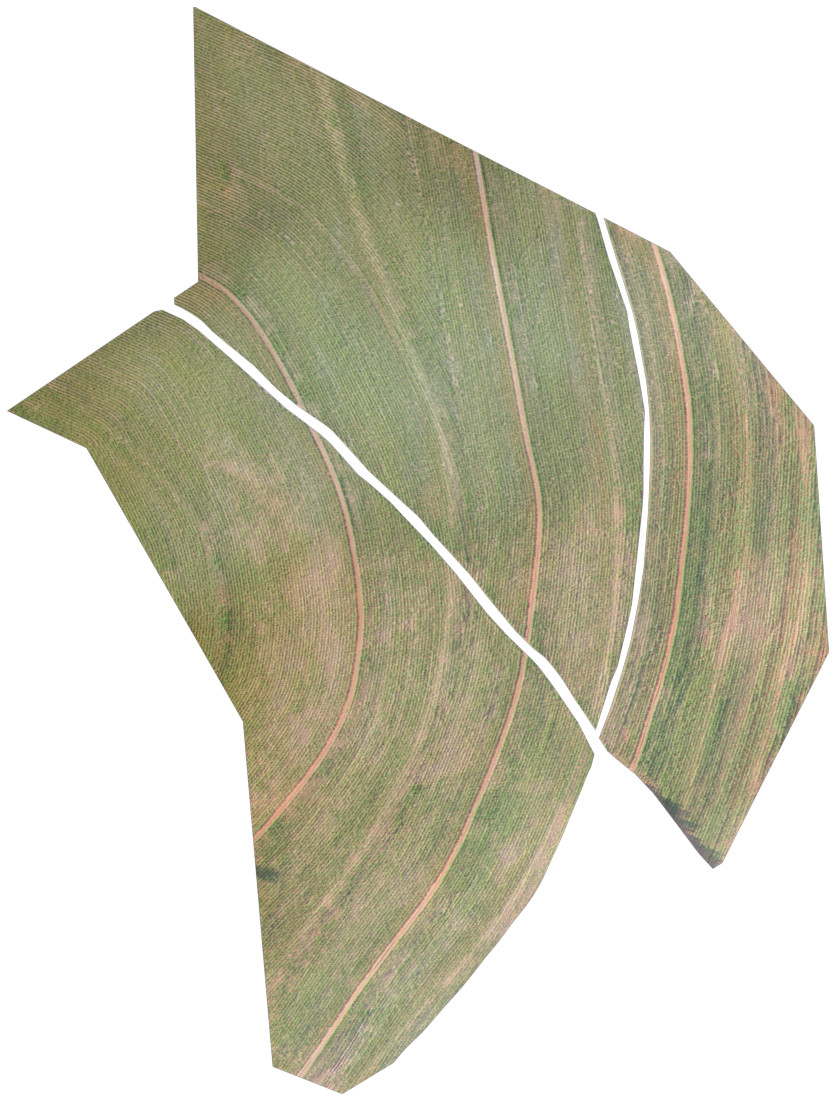
\includegraphics[width=0.11\textwidth]{img/a2.jpg}} 
    \subfigure[]{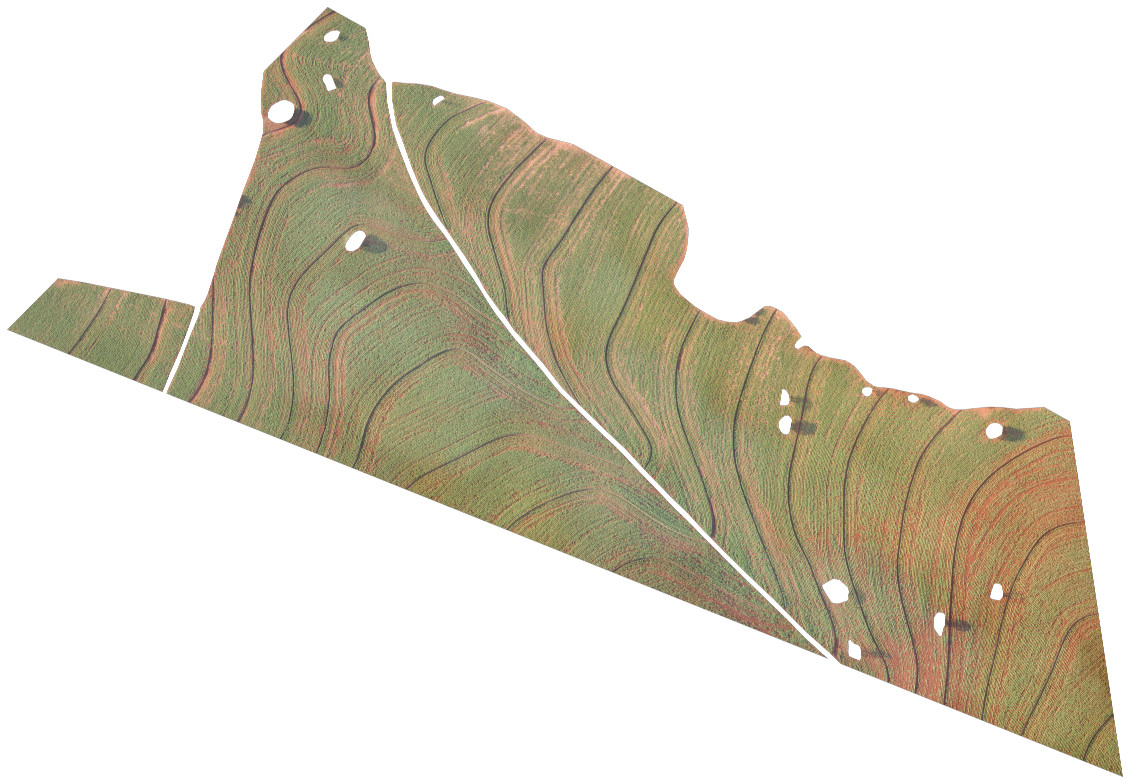
\includegraphics[width=0.32\textwidth]{img/b2.jpg}} 
    \subfigure[]{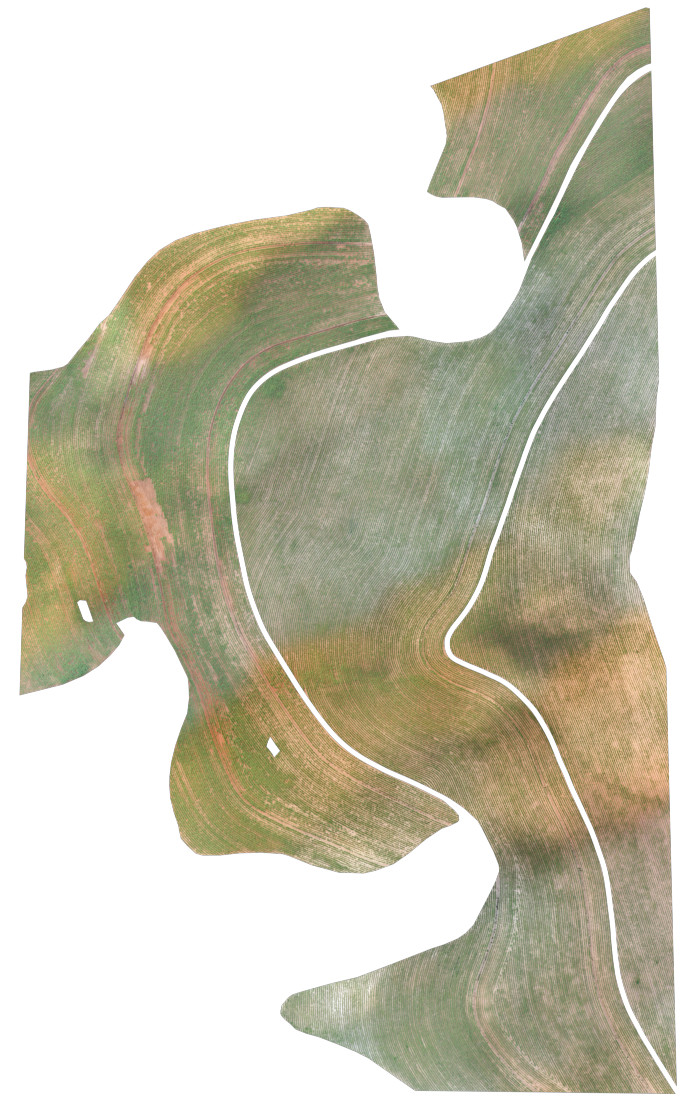
\includegraphics[width=0.14\textwidth]{img/c2.jpg}}
    \subfigure[]{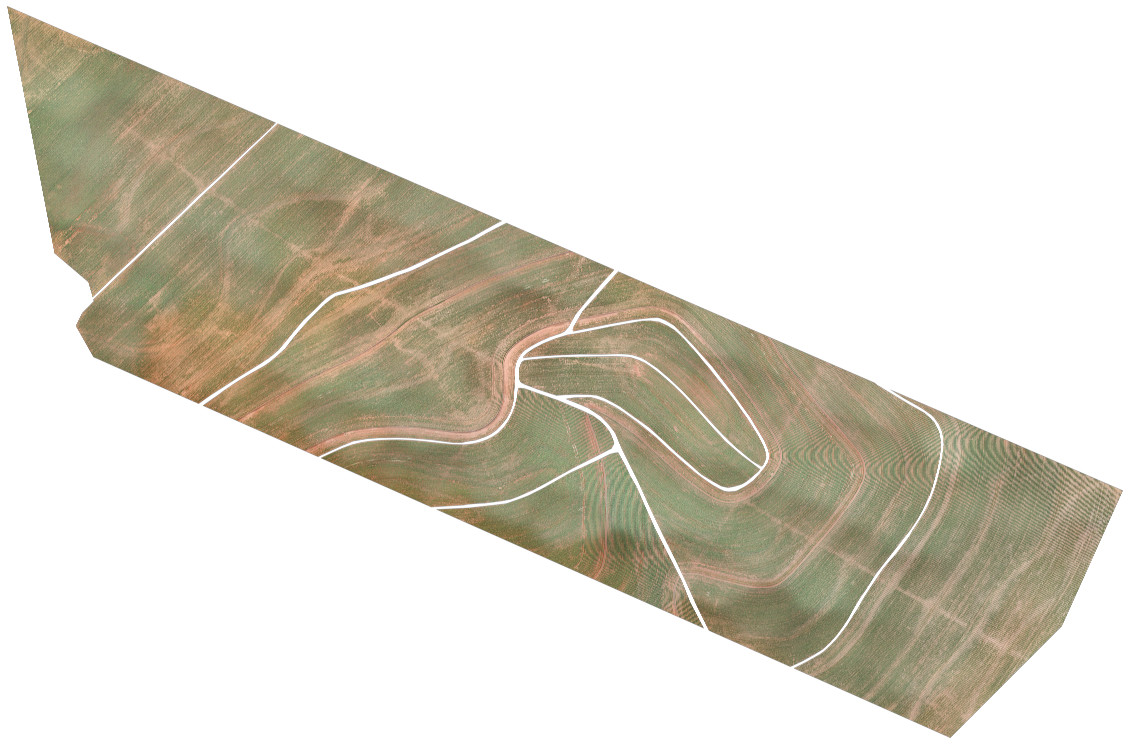
\includegraphics[width=0.40\textwidth]{img/d2.jpg}}
    \caption{Mosaicos e seus respectivos tamanhos: (a) 11180 $\times$ 8449; (b) 16677 $\times$ 24181; (c) 17497 $\times$ 10771; (d) 19833 $\times$ 30255.}
    \label{fig:mosaicos1}
\end{figure}

\begin{figure}[htbp]
    \centering
    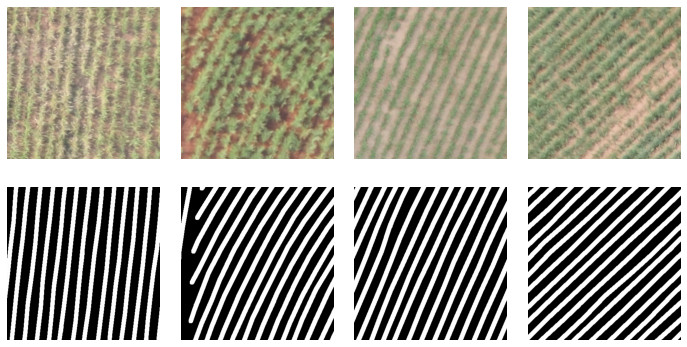
\includegraphics[width=0.8\textwidth]{img/linhas2.jpg}
    \caption{Exemplos de marcações feitas pelo especialista nos 4 mosaicos em \citeonline{Silva_2020}.}
    \label{fig:linhas}
\end{figure}

Em \citeonline{Pereira_Junior_2020}, utilizaram 1 mosaico \cite{CropRowsDataset2019} (\autoref{fig:mosaicos2}) capturado com uma câmera RGB \textit{Canon G9X} e VANT \textit{Horus Aeronaves}, resultando em um GSD aproximado de 5 cm. O mosaico foi marcado por um especialista; as linha de plantio em verde, o fundo/solo em vermelho, já fora do mosaico todos pixels foram definidos como pretos.

\begin{figure}[htbp]
    \centering
    \subfigure[]{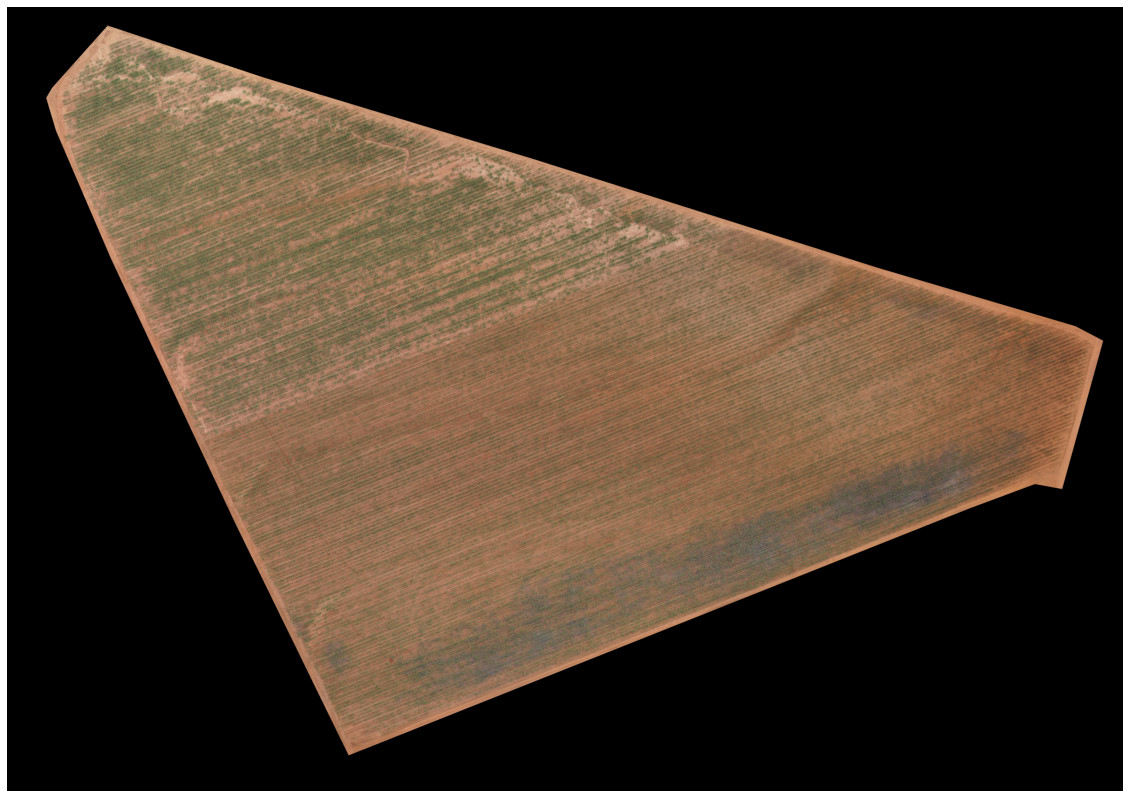
\includegraphics[width=0.49\textwidth]{img/sugarcane1-s2.jpg}} 
    \subfigure[]{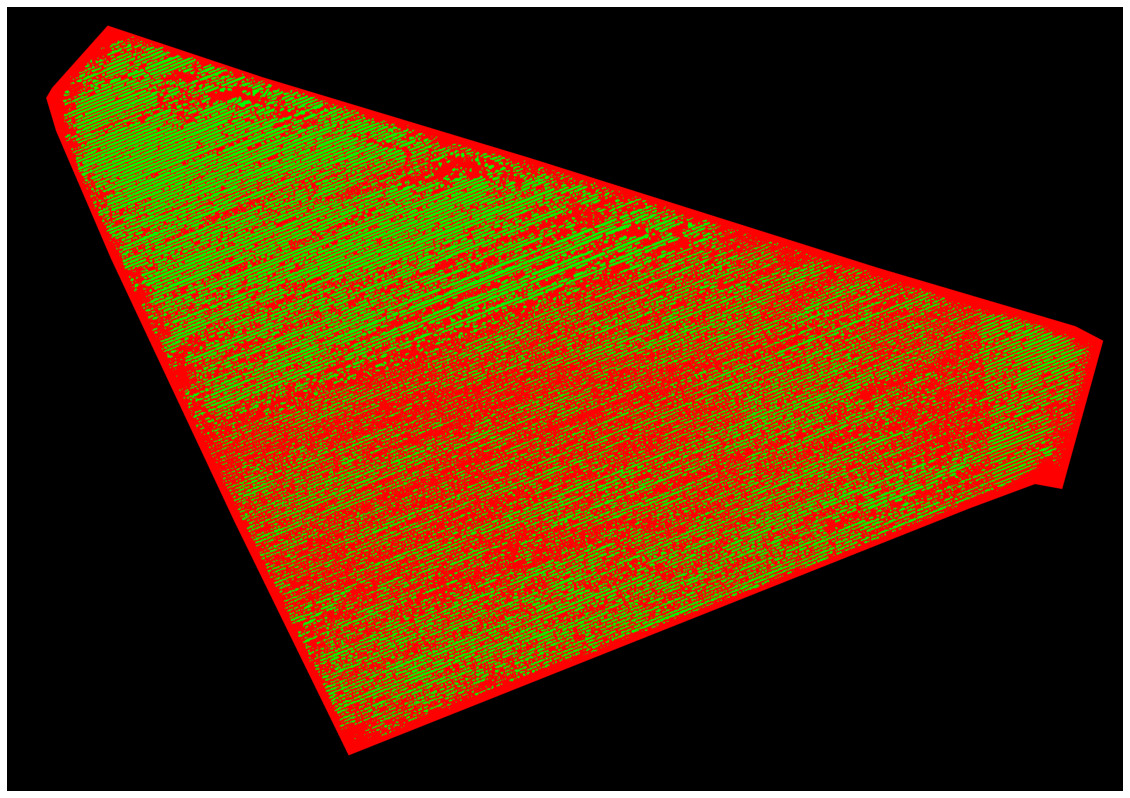
\includegraphics[width=0.49\textwidth]{img/sugarcane1-GT-s2.jpg}} 
    \caption{Mosaico \citeonline{CropRowsDataset2019} (a) mosaico de tamanho (incluindo bordas pretas) 6595 $\times$ 9391; (b) marcação do especialista (de mesmo tamanho).}
    \label{fig:mosaicos2}
\end{figure}

Além dos dois \textit{datasets} disponíveis, imagens/mosaicos devem ser capturados, dependendo da demanda dos experimentos, de culturas de cana-de-açúcar e outras, através dos VANTs. Depois sendo feita a marcação por um especialista, destacando as linhas de plantio do solo/fundo.

\dotsBlue

\subsection{Pré-processamento}

No pré-processamento ajustes serão feitos nas imagens de modo a facilitar ou melhorar os resultados da segmentação. Dentre eles a correção de brilho e contraste, quando forem necessário. Além da remoção de ruídos que podem estar presentes nas imagens. Após converter as imagens para níveis de cinza, as operações morfológicas podem ser úteis.

A dilatação pode ser utilizada para juntar plantas isoladas de suas respectivas linhas de plantio devido a pequenas falhas, assim expandir extremidades e conectar elas com a linha de plantio. Por outro lado, a erosão, pode ser utilizada para separar estreitos e compridos filamentos onde plantas podem estar ligadas com outras linhas de plantio ou com uma errada.

\dotsBlue

\subsection{Segmentação}

O processamento principal, as vezes também chamado de segmentação é uma das partes mais importantes do PDI. Para esse projeto, inicialmente, foi escolhido redes neurais para segmentar as imagens das linhas de plantio. Elas podem ter bom resultado na segmentação, em comparação com os algoritmos tradicionais (e outros métodos como AG), por utilizar não apenas o tom avermelhado do solo e esverdado da plantas, mas outras características que elas conseguem extrair das imagens. Dentre essas características, podem ser contornos, formatos de linhas, outros tipos de formatos específicos. 

\dotsBlue

\subsection{Pós-processamento}

O pós-processamento é responsável por refinar a segmentação obtida na etapa anterior. Aqui também será refinado as linhas detectadas, por exemplo, utilizando a TR ou a TH. Além de tratar as linhas de plantio com formato de linhas retas e linhas curvas. Também pode ser utilizado as operações morfológica para juntar ou separar finos filamentos.

\dotsBlue

\subsection{Avaliação dos resultados}

Para avaliação dos resultados é importante ter um método confiável e de fácil replicação/teste. Por isso as marcações por especialistas são tão importantes. Neste projeto será comparado as marcações feitas pelos especialistas com as linhas de plantio detectadas nas etapas anteriores. Para comparar os resultados será utilizado o Coeficiente de \textit{Dice} (CD), (como em \citeonline{Silva_Escarpinati_Backes_2021}). Com o CD é possível comparar o quão similar duas imagens binárias são. Considerando A e B como imagens binárias, o CD é definido por:

\begin{equation}
    CD = 2 \frac{|A \cap B|}{|A| + |B|}
\end{equation}

No resultado de CD, $0 \le CD \ge 1$, quanto mais próximo de 1, mais similar são as imagens A e B. Para a validação dos resultados serão utilizadas imagens de vários hectares de cana-de-açúcar contendo diferentes idades e tamanhos de plantas. Nesta validação, assume-se que o resultado gerado pelo especialista, sua marcação, de forma manual é o melhor resultado esperado. Assim quanto mais próximo deste resultado as imagens geradas pelos métodos propostos estiverem, mais assertivas elas serão consideradas.

\dotsBlue

\section{Resultados esperados}
% => Liste os resultados mais importantes que você pretende obter a partir de seu trabalho de doutorado.

Ao fim do projeto, espera-se obter um método de avaliação automática capaz de realizar de forma mais eficiente e com maior precisão o processo de segmentação de imagens de linhas de plantio da cultura de cana-de-açúcar. O projeto é focado em imagens de VANTs, diferentes de outros trabalhos que utilizam imagens de satélites e, principalmente, de baixíssimas altitudes (tiradas do solo ou acopladas em maquinário agrícola). As técnicas estudas e desenvolvidas serão utilizadas em sua melhor combinação para detectar as linhas de plantio.

Também é esperado que este método consiga lidar bem com linhas de plantio em formato de linhas retas e linhas curvas nas plantações de cana-de-açúcar em vários estágios (idades diferentes)

\dotsBlue


%\section{Esquema Geral do Texto da Dissertação (opcional)}
% => Descreva o “esqueleto” de sua dissertação, como vai estruturar os capítulos e seções. Dê um título, mesmo que provisório, a sua dissertação.

\section{Cronograma de execução}
% => Detalhe o cronograma das principais etapas de seu trabalho finalizando pela data da defesa.

Para cumprir os objetivos descritos, o plano de pesquisa foi dividido em atividades e seus respectivos meses. O cronograma de atividades do projeto pode ser visualizado na \autoref{tab:cronograma}, onde está definida a
duração das principais atividades.

\begin{table}[htb]
\centering
\caption{Cronograma de atividades}
\label{tab:cronograma}
\begin{tabular}{|c|c|c|c|c|c|c|c|c|c|c|c|c|c|c|c|c|}
\hline
          & \multicolumn{2}{c|}{2021} & \multicolumn{12}{c|}{2022}                    & \multicolumn{2}{c|}{2023} \\ \hline
Atividade & N           & D           & J & F & M & A & M & J & J & A & S & O & N & D & J           & F           \\ \hline
A1        & X           & X           & X & X &   &   &   &   &   &   &   &   &   &   &             &             \\ \hline
A2        &             &             & X & X & X & X &   &   &   &   &   &   &   &   &             &             \\ \hline
A3        &             &             &   &   & X & X & X &   &   &   &   &   &   &   &             &             \\ \hline
A4        &             &             &   &   &   & X & X & X &   &   &   &   &   &   &             &             \\ \hline
A5        &             &             &   &   &   &   & X & X & X &   &   &   &   &   &             &             \\ \hline
A6        &             &             &   &   &   &   &   & X & X & X &   &   &   &   &             &             \\ \hline
A7        &             &             &   &   &   &   &   &   & X & X &   &   &   &   &             &             \\ \hline
A8        &             &             &   &   &   &   &   &   &   & X & X & X &   &   &             &             \\ \hline
A9        &             &             &   &   &   &   &   &   &   &   &   & X & X & X & X           &             \\ \hline
A10       &             &             &   &   &   &   &   &   &   &   &   &   &   &   & X           & X           \\ \hline
\end{tabular}
\end{table}

As atividades são descritas abaixo:

\begin{itemize}
    \item A1: revisão bibliográfica sobre os métodos de segmentação e detecção de linhas de plantio.
    \item A2: estudo dos algoritmos e métodos encontrados na literatura correlata sobre segmentação de imagens.
    \item A3: estudo dos algoritmos e métodos encontrados na literatura correlata sobre \textit{deep learning} na segmentação de imagens.
    \item A4: avaliação dos algoritmos estudados com relação a possibilidade de aplicar as técnicas estudadas no contexto do nosso trabalho.
    \item A5: aplicação e análise dos algoritmos e métodos encontrados em imagens reais.
    \item A6: avaliação dos resultados e propostas de melhorias.
    \item A7: readequação dos parâmetros e mais experimentos (caso necessário).
    \item A8: elaboração e submissão de artigos científicos para periódicos e/ou congresso da área.
    \item A9: elaboração da dissertação (escrita e preparação para a defesa).
    \item A10: defesa da dissertação.
\end{itemize}

% \section{Justificativa pelo atraso na entrega do projeto (tópico obrigatório somente no caso de entrega do projeto foram do prazo regulamentar*)}
% => Descrever as justificativas que levaram ao atraso na entrega do projeto.

% \textbf{*RI-PPGCO/UFU, art. 18, parágrafo único:
% O projeto de Dissertação de Mestrado deverá ser apresentado pelo estudante até o final do segundo semestre letivo, contado a partir da matrícula de ingresso como aluno regular.}

\bigskip
\noindent \boxYellow{Uberlândia, 10 de novembro de 2021.}
% Encaminhar para o e-mail cpgfacom@ufu.br

% \section{Bibliografia}
\bibliography{references}

\end{document}
